\documentclass[12pt]{exam}

\usepackage[utf8]{inputenc}  % For UTF8 source encoding.
\usepackage{amsmath}  % For displaying math equations.
\usepackage{amsfonts} % For mathematical fonts (like \mathbb{E}!).
\usepackage{upgreek}  % For upright Greek letters, such as \upvarphi.
\usepackage{wasysym}  % For additional glyphs (like \smiley!).
\usepackage{mathrsfs} % For script text (hash families and universes).
\usepackage{enumitem}
\usepackage{graphicx}
% For document margins.
\usepackage[left=.8in, right=.8in, top=1in, bottom=1in]{geometry}
\usepackage{lastpage} % For a reference to the number of pages.
\usepackage[table,xcdraw]{xcolor}
\usepackage{pdfpages}
\usepackage{verbatim}

% TODO: Enter your name here :)
\newcommand*{\authorname}{Luis A. Perez}

\newcommand*{\duedate}{Wednesday, July 17th}
\newcommand*{\duetime}{11:59 pm}

% Fancy headers and footers
\headrule
\firstpageheader{EE 263\\Summer 2019}{Homework 3 \\ }{Due: \duedate\\at \duetime}
\runningheader{EE 263}{Homework 3}{\authorname}
\footer{}{\footnotesize{Page \thepage\ of \pageref{LastPage}}}{}

% Exam questions.
\newcommand{\Q}[1]{\question{\large{\textbf{#1}}}}
\qformat{}  % Remove formatting from exam questions.

% Useful macro commands.
\newcommand*{\bigtheta}[1]{\Theta\left( #1 \right)}
\newcommand*{\bigo}[1]{O \left( #1 \right)}
\newcommand*{\bigomega}[1]{\Omega \left( #1 \right)}
\newcommand*{\prob}[1]{\text{Pr} \left[ #1 \right]}
\newcommand*{\ex}[1]{\text{E} \left[ #1 \right]}
\newcommand*{\var}[1]{\text{Var} \left[ #1 \right]}

\newcommand*{\norm}[1]{\left\lVert #1 \right\rVert}
\newcommand*{\HH}{\mathscr{H}}   % Family of hash functions.
\newcommand*{\UU}{\mathscr{U}}   % Universe.
\newcommand*{\eps}{\varepsilon}  % Epsilon.


% Custom formatting for problem parts.
\renewcommand{\thepartno}{\roman{partno}}
\renewcommand{\partlabel}{\thepartno.}

% Framed answers.
\newcommand{\answerbox}[1]{
\begin{framed}
\hspace{\fill}
\vspace{#1}
\end{framed}}

\printanswers

\setlength\answerlinelength{2in} \setlength\answerskip{0.3in}

\begin{document}
\title{EE 263 Homework 3}
\author{\authorname}
\date{}
\maketitle
\thispagestyle{headandfoot}
\setcounter{MaxMatrixCols}{15}

\begin{questions}
%%%%%%%%%%%%%%%%%%%%%%%%%%%%%%%%%%%
\Q{Memory of a linear dynamical, time-invariant system}

  \begin{solution}
    \begin{enumerate}[label=(\alph*)]
      \item Let us first consider how we might check if a valid impose response of fixed size $M$ exists. The first thing to note is that the covolution operator given in the problem statent can actually be written as a linear system:
      \[
        \bar{y} = Ah
      \]
      where $\bar{y} \in \mathbb{R}^{T - M}, h \in \mathbb{R}^{M}$ and $A \in \mathbb{R}^{(T-M) \times M}$. Note that we remove the first $\{y_1, \cdots, y_{M}\}$. In fact, we can use the matrix $A$ as defined below:
      \begin{align*}
        A &=
          \begin{bmatrix}
          u_M & u_{M-1} & u_{M-2} & \cdots & u_1 \\ 
          u_{M+1} & u_{M} & u_{M-1} & \cdots & u_2 \\ 
          u_{M+2} & u_{M + 1} & u_{M} & \cdots & u_2 \\ 
          \vdots & \vdots & \vdots & \ddots \\
          u_{T-2} & u_{T-3} & u_{T-4} & \cdots & u_{T-M-1} \\
          u_{T-1} & u_{T-2} & u_{T-3} & \cdots & u_{T-M} \\
          \end{bmatrix} \\
        y_{-1} &= 
          \begin{bmatrix}
            y_{M+1} \\
            \vdots \\
            y_T
          \end{bmatrix} \\
        h &= 
          \begin{bmatrix}
            h_1 \\
            \vdots \\
            h_M
          \end{bmatrix}
      \end{align*}
      We can see by inspection above that $Ah$ performs the needed convolutions betweens $u$ and $h$ to obtain $\bar{y}$, by the properties of matrix multiplication (eg, to obtain $y_i$, we compute the dot product of the $i-M$-th row of $A$ with $h$, which is exactly what our convolution dictates, and for $i \leq M$, the convolution is not fully defined so we ignore them).

      In the problem statement, we're given the fact that $T > 2M$, so this means that there will always be at least $T-M > 2M -M = M$ rows in $A$, meaning it will always be a tall and skinny matrix. 

      As such, we can use the pseudo inverse to find the closests solution for $h$, computing:
      \[
        \bar{h} = (A^TA)^{-1}A^T\bar{y}
      \]
      Finally, once we've computed this $h$, we can re-compute that $\bar{y}$ given our inputs forming $A$, and see if this equals our what we started with. In other words, we have that:
      \[
        ||A\bar{h} - \bar{y}|| \leq \epsilon \implies M \text{ is a valid value} \tag{$\epsilon$ is needed to deal with floating point imprecision}
      \]
      The above gives us a way to check if $M$ is sufficient. To finallize our method, we simply iterate over the possible values of $M$ from $M = 1, \cdots \frac{T}{2} - 1$ in order until we find a valid value.

      \item Applying the process we described above, we find that $M = 7$ is the smallest value that works. We also have:
      \[
        h =
          \begin{bmatrix}
            0.63 \\
            0.27 \\
            0.02 \\
            0.37 \\
            0.96 \\
            0.95 \\
            0.46
          \end{bmatrix}
      \]
    \end{enumerate}
  \end{solution}

\newpage
\Q{Norm preserving implies orthonormal columns}

  \begin{solution}
    We show that if $A \in \mathbb{R}^{m \times n}$ satifies $|| Ax|| = ||x||$ for all $x \in \mathbb{R}^n$, then $A$ has orthonormal columns.

    This boils down to showing that $A^TA = I$, which can be broken into two parts. Let $A_i$ be the $i$-th column of $A$. Then we need to show that $A_i^TA_i = 1$, and that $A_i^TA_j = 0$ for $i \neq j$. Let us consider the former first:

    \begin{align*}
      A_i^TA_i &= (Ae_i)^T(Ae_i) \tag{Multiplying $A$ by $e_i$ extracts the $i$-th column} \\
      &= ||Ae_i||^2 \tag{Definition of dot product treating $Ae_i$ as a vector} \\
      &= ||e_i||^2 \tag{Multiplication by $A$ preserves the norm} \\
      &= 1
    \end{align*}
    Let us now consider the latter case. We follow the hint:
    \begin{align*}
    ||A(e_i + e_j)||^2 &= ||e_i + e_j|| \tag{$A$ preserves norm} \\
    &= 2
    \end{align*}
    However, we also have that:
    \begin{align*}
    ||A(e_i + e_j)||^2 &= ||Ae_i + Ae_j||^2 \tag{Linearity of $A$} \\
    &= ||Ae_i||^2 + ||Ae_j||^2 + 2(Ae_i)^T(Ae_j) \tag{Definition of vector norm} \\
    &= 2 + 2(Ae_i)^T(Ae_j) \tag{Using previous results}
    \end{align*}
    Putting the two results together, we must have that:
    \begin{align*}
      2 + 2(Ae_i)^T(Ae_j) = 2 \implies 2(Ae_i)^T(Ae_j) = 0 \implies (Ae_i)^T(Ae_j) = 0 \implies A_i^TA_j = 0
    \end{align*}
    As such, we've now shown that $A^TA = I$.
  \end{solution}


\newpage
\Q{Sensor integrity monitor}
  \begin{solution}
    We need to find $k \in \mathbb{R}^{k \times m}$ such that:
      \begin{itemize}
        \item $By = 0$ for any $y$ which is consistent.
        \item $By \neq 0$ for any $y$ which is inconsistent.
      \end{itemize}

    The above can be summarized as follow. Requirement (1) means that given $y \in \textbf{Img}(A)$, we must have $By = 0$. This means that $\textbf{Img}(A) \subseteq \textbf{Ker}(B) $.

    The second requirement specifies that for any $y \notin \textbf{Img}(A)$, we must have $By \neq 0$. Phrase another way, this says that if $By = 0$, it must be in the $\textbf{Img}(A)$. So we have $\textbf{Ker}(B) \subseteq \textbf{Img}(A)$.

    As such, we're really just tring to construct a matrix $B$ whose kernal is equal to the span of of the columns of $A$. This is actually a rather straight-forward process as long as we recall the following theorem, which holds for \textit{any} matrix $C$:

    \[
      \textbf{Ker}(C^T) = \textbf{Img}(C)^{\perp}
    \]
    Thinking about it step-by-step, if the Kernel of $B$ is equal to the Image of $A$, it must mean that the Image of $B$ is equal to the complement of the Image of $A$. Using the formula presented abouve, the completement of the Image of $A$ is the null-space of of $A^T$.

    So simply put, we just need to (1) find the $M-N$ vectors spanning the nullspace of $A^T$ and take these to be the rows of $B$. This will guarantee that the Kernel of $B$ will equal the image of $A$.

    Doing exactly the process described above gives us $B \in \mathbb{R}^{2 \times 5}$ as follows:

    \[
      B =
        \begin{bmatrix}
          0 & -5.47259193 &  2 &  8.47259193 & 1 \\
          0 & 6.97831636 & 6.39848918 & 2.61941742 & 3.19924459
        \end{bmatrix}
    \]


  \end{solution}

\newpage
\Q{Coin Collector Robot}
  \begin{solution}
    \begin{enumerate}[label=(\alph*)]
      \item To find the coordinates of the robot at time $t$, we have to consider what the effect of the constant force is. Given that the robot is unit mass, we have $a_i = f_i$ (acceleration is equal to the force).

      Let us now consider the effect of the force $f_i$ for one second (from $t = 2i -2$ to $t = 2i - 1$) on the final position:
      \[
        \Delta x_i^1 = \underbrace{\frac{1}{2}f_i}_{\text{Change caused by acceleration over 1 second}} + \underbrace{f_i(t - (2i - 1))}_{\text{Change caused by change in velocity}}
      \]
      As such, for all $f_i$ that are applied over the full two second period, we will have:
      \[
        \Delta x_i = \underbrace{2f_i}_{\text{Change caused by acceleration over 2 seconds}} + \underbrace{2f_i(t - 2i)}_{\text{Change caused by change in velocity}}
      \]
    The final position at time $t$, let's call it $x_t$, will then be given by $x_t = x_0 + \Delta x$ where $\Delta x$ (the total change) can be computed with the following:
    \begin{align*}
      \Delta x &= 
        \begin{cases}
          \sum_{i=1}^{\frac{t}{2} } \Delta x_i  & t \text{ is even} \\
          \Delta x_{\frac{t+1}{2}}^1 + \sum_{i=1}^{\frac{t-1}{2} } \Delta x_i & t \text{ is odd}
        \end{cases}
    \end{align*}
    Furthermore, we know that $x_0 = 0$. As such, the postion at time $t$ is given by $(x_t, y_t)$ where 
    \begin{align*}
      y_t &= t \\
      x_t &=
        \begin{cases}
          \sum_{i=1}^{\frac{t}{2}} 2f_i + 2f_i(t - 2i) & t \text{ is even} \\
          \frac{1}{2}f_{\frac{t+1}{2}} + \sum_{i=1}^{\frac{t-1}{2}} 2f_i + 2f_i(t - 2i) & t \text{ is odd}
        \end{cases}
    \end{align*}
    We note that the above are all linear relations, so if we were so inclined, we could re-write the above as simply $x_t = c_t^T f$ for some vector $c_t \in \mathbb{R}^{n}$ and $f = \begin{bmatrix} f_1 \\ f_2 \\ \vdots\\ f_n \end{bmatrix}$. In fact, we have:
    \begin{align*}
      c_t &=
        \begin{bmatrix}
          2 + 2(t -2) \\
          2 + 2(t - 4) \\
          2 + 2(t - 6) \\
          \vdots \\
          2 + 2(6) \\
          2 + 2(4) \\
          2 + 2(2) \\
          2 \\
          0 \\
          0 \\
          \vdots
        \end{bmatrix} \in \mathbb{R}^n \tag{$t$ is even} \\
        c_t &=
        \begin{bmatrix}
          2 + 2(t -2) \\
          2 + 2(t - 4) \\
          2 + 2(t - 6) \\
          \vdots \\
          2 + 2(5) \\
          2 + 2(3) \\
          2 + 2(1) \\
          \frac{1}{2} \\
          0 \\
          0 \\
          \vdots
        \end{bmatrix} \in \mathbb{R}^n \tag{$t$ is odd} 
    \end{align*}
      \item 
        We are now given a sequence $(x_1, y_1), \cdots, (x_{2n}, y_{2n})$ of $2n$ coins, and we want to determine whether the robot can collect them. For simplicitly, we assume that $y_i = i$ (all we require is that $i \neq j \implies y_i \neq y_j$, since if this were not the case, it's immediate that the coins cannot be collected, but the problem can be presented more simply if we have $y_i = i$).

        From our work in part (a), we know that the robot can collect the coins if the following all hold:
        \begin{align*}
          x_1 &= c_1^T f \\
          x_2 & = c_2^T f \\
          \vdots \\
          x_{n-1} & c_{n-1}^T f \\
          x_n &= c_n^T f
        \end{align*}
        which we can write as the linear system $x = Af$ where $x \in \mathbb{R}^{2n}, f \in \mathbb{R}^n$ and $A \in \mathbb{R}^{2n \times n}$ as per the below:
        \[
          \begin{bmatrix}
            x_1 \\
            x_2 \\
            \vdots \\
            x_{2n}
          \end{bmatrix} =
          \begin{bmatrix}
            & \text{---} & c_1^T &\text{---}  & \\
            &\text{---} & c_2^T &\text{---}  & \\
            & & \vdots & & \\
            &\text{---} & c_{2n}^T &\text{---}  &
          \end{bmatrix}
          \begin{bmatrix}
            f_1 \\
            f_2 \\
            \vdots \\
            f_n
          \end{bmatrix}
        \]
        As such, we have an overdetermined system of equations. As such, we can compute the closests fit $\hat{f}$:
        \[
          \hat{f} = (A^TA)^{-1}A^Tx
        \]
        and check to see if this $\hat{f}$ satisfies our problem statement. In other words, to check feasibility, we need to check if:
        \[
          || A\hat{f} - x|| < \eps
        \]
        forms some sufficiently small $\eps$ (due to floating point imprecision).
      
      \item See attached code. We show that for the data from ``robot\_coin\_collector.m'', not all the coins can be collected under this framework.
      
      \item If we now that only one of the coins cannot be collected, we can simply, we can simply attempt the same process above but with $A_{-i}$ and $x_{-i}$ (eg, we remove the $i$-th row from $A$ and remove the $i$-th element from $x$. This then imposes no restrictions on the robot for time $i$ in the x-position, which relaxes our system.

      If we check for all of $i = 1, \cdots, 2n$, we will be able to determine if the robot can collect all but one of the coins (and can even identify the coin).

      \item See attached code where the process described above is implemented.

      It turns out that the 7-th coin (1-indexed) is the coin which cannot be collected. More specifically, the bad coin is $(x_7, y_7) = (13.0, 7)$.

      In order to collect the remaning $2n - 1$ coins, the forces applied must be:
      \[
        f =
          \begin{bmatrix}
            1 \\
            -4 \\
            7 \\
            -10 \\
            20 \\
            -35
          \end{bmatrix}
      \]
      We plot the coin and the robot locations in Figure \ref{fig:robot_collector}.
    \end{enumerate}
  \end{solution}

  \begin{figure}
    \centering
    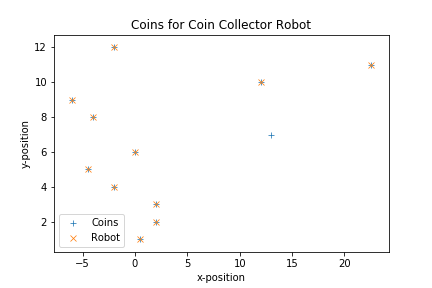
\includegraphics{figures/robot_collector.png}
    \caption{Location of coins and robot with the applied forces $f$}
    \label{fig:robot_collector}
  \end{figure}

\newpage
\Q{Solving linear equations via QR Factorization}

  \begin{solution}
    The problem statement essentially boils down to solving the system $Rx = z$ where $R \in \mathbb{R}^{n \times n}$ is upper triangular and non-singular (eg, $R_{ii} \neq 0, \forall i$) and $z,x \in \mathbb{R}^n$.

    The algoritm proceeds as follows:
    \begin{enumerate}
      \item First, let us find $x_n$. Let $R_i \in \mathbb{R}^{1 \times n}$ be the $i$-th row of $R$ as a row vector. We have:
        \begin{align*}
          z_n &= R_n x \\
          &= \sum_{i=1}^n R_{ni} x_i \\
          &= R_{nn} x_n \tag{Since $R$ is upper triangular, $R_{ni} = 0$ for $i < n$} \\
          \implies x_n &= \frac{z_n}{R_{nn}} \tag{Note this is valid since $R_{nn} \neq 0$}
        \end{align*}
      \item Using a similar process, we can now find $x_{n-1}$. We have:
        \begin{align*}
          z_{n-1} &= R_{n-1} x \\
          &= \sum_{i=1}^n R_{n-1,i} x_i \\
          &= R_{n-1, n-1}x_{n-1} + R_{n-1,n} x_n \tag{Since $R$ is upper triangular, $R_{n-1,i} = 0$ for $i < n-1$} \\
          \implies x_{n-1} &= \frac{z_n - R_{n-1,n}x_n}{R_{n-1,n}} \tag{Note this is valid since $R_{n-1,n} \neq 0$}
        \end{align*}
        While the equation above looks more complicated, we note that all of the variables in the RHS are known (specifically, we found the value of $x_n$ previously).
      \item We simply continue the process from above. Let us assume that we've found the values $x_k$ for all $k > i$. Then to compute $x_i$ (the next value), we have:
        \begin{align*}
          z_i &= R_i x \\
          &= \sum_{j=1}^n R_{ij} x_j \\
          &= \sum_{j=i}^n R_{ij} x_j\tag{Since $R$ is upper triangular, $R_{ij} = 0$ for $j < i$} \\
          \implies x_i &= \frac{z_i - \sum_{j=i+1}^n R_{ij} x_j}{R_{ii}} \tag{Note this is valid since $R_{ii} \neq 0$}
        \end{align*}
        We know $z_i, R_{ij}, \forall j$, and by our assumption, we know $x_k, \forall k > i$, so we know all the variables in the LHS. As such, it's relatively straight-forwrad to compute $x_i$.
    \end{enumerate}

    As such, we can see that the $x_n, x_{n-1}, \cdots, x_1$ produced by our algorithm are valid solutions to the system $z = Rx$. Furthermore, the algorithm cannot fail since $R$ is non-singular (all diagonal entries are non-zero).
  \end{solution}

\newpage
\Q{Quadratic extrapolation of a time series, using least-squares fit}
  \begin{solution}
  \begin{enumerate}[label=(\alph*)]
    \item In the problem statement, we are given that $\hat{z}(t+1) = f(t+1)$ where $f(\tau) = a_2\tau^2 + a_1 \tau + a_0$ is the quadratic function which minimizes:
    \[
      J = \sum_{\tau = t-9}^t (z(\tau) - f(\tau))^2
    \]
    We can rewrite the above in matrix form as follows:
    \[
      J = ||Fa - z||^2
    \]
    where 
    \begin{align*}
      z &=
        \begin{bmatrix}
          z(t) \\
          z(t-1) \\
          \vdots \\
          z(t-9)
        \end{bmatrix} \\
      a &= 
        \begin{bmatrix}
          a_1 \\
          a_2 \\
          a_3
        \end{bmatrix} \\
      F &=
        \begin{bmatrix}
          1 & t & t^2 \\
          1 & t - 1 & (t-1)^2 \\
          \vdots & \vdots & \vdots \\
          1 & t - 9 & (t - 9)^2
        \end{bmatrix}
    \end{align*}
    If we want to solve for $a$, we can immediately arrive at the solution (based on what we've covered in lecture):
    \[
      a = (F^TF)^{-1}F^Tz
    \]
    With the above, we can write $\hat{z}(t+1)$ as follows:
    \begin{align*}
      \hat{z}(t+1) &= f(t+1)  \\
      &= a_1 + a_2(t+1) + a_3(t+1)^2 \\
      &=
        \begin{bmatrix}
          1 & t + 1 & (t+1) 
        \end{bmatrix}
        \begin{bmatrix}
          a_1 \\
          a_2 \\
          a_3
        \end{bmatrix}\\
      &= 
        \begin{bmatrix}
          1 & t + 1 & (t+1) 
        \end{bmatrix}(F^TF)^{-1}F^Tz
    \end{align*}
    As such, we can see that for a given value of $t$, we have:
    \[
      \hat{z}(t+1) =
        \begin{bmatrix}
          1 & t + 1 & (t+1)^2
        \end{bmatrix} (F^TF)^{-1}F^T
        \begin{bmatrix}
          z(t) \\
          z(t-1) \\
          \vdots \\
          z(t-9)
        \end{bmatrix}
    \]
    which implies that we should have:
    \[
      c =  \begin{bmatrix}
          1 & t + 1 & (t+1)^2
        \end{bmatrix} (F^TF)^{-1}F^T
    \]
    which at first glance appears to depend on the value of $t$. However, using code to solve the system symbolically, we see that $c$ does not vary with time, and is infact given by the constant matrix:
    \begin{align*}
      c &=
        \begin{bmatrix}
          \frac{9}{10} & \frac{1}{2} & \frac{11}{60} & -\frac{1}{20} & -\frac{1}{5} & -\frac{4}{15} & -\frac{1}{4} & -\frac{3}{20} & \frac{1}{30} & \frac{3}{10}
        \end{bmatrix} \\
        &=
          \begin{bmatrix}
            0.9       &   0.5       &   0.18333333&  -0.05      &  -0.2       &  -0.26666667&  -0.25      &  -0.15      &   0.03333333&   0.3 
          \end{bmatrix}
    \end{align*}
    \item See attached code for details on how we calculate the RMS. The final result is an RMS of:
    \[
      0.050960852617736675
    \]
    \item We plot the requested serieses in Figure \ref{fig:estimated_time_series}. There is no previous problem using inteporlation on the previous three values (as far as we are aware), so we cannot comment on the RMS.
  \end{enumerate}

  \end{solution}

  \begin{figure}[!ht]
    \centering
    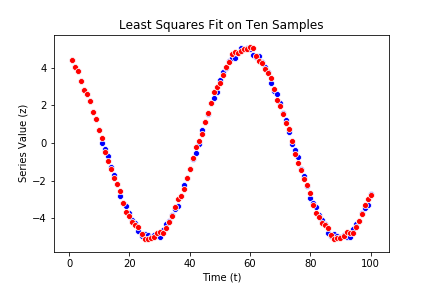
\includegraphics{figures/least_squares_fit_series.png}
    \caption{In red is the estimated values $\hat{z}$ using the model described in part (a) of the homework. In blue is the real values of the series, $z$.}
    \label{fig:estimated_time_series}
  \end{figure}



\newpage
\Q{Householder reflection}
  \begin{solution}
  Not required.
  \end{solution}



\newpage
\Q{Vector space multiple access}
  \begin{solution}
  Not required.
  \end{solution}
\end{questions}


















\end{document}
